\documentclass[twoside, letterpaper, 12pt]{report}
\usepackage{orthodoxservicebook}

\title{The Sunday Reader's Service of the \\ \textsc{Typica} \\ 2020 July 26}
\titlepic{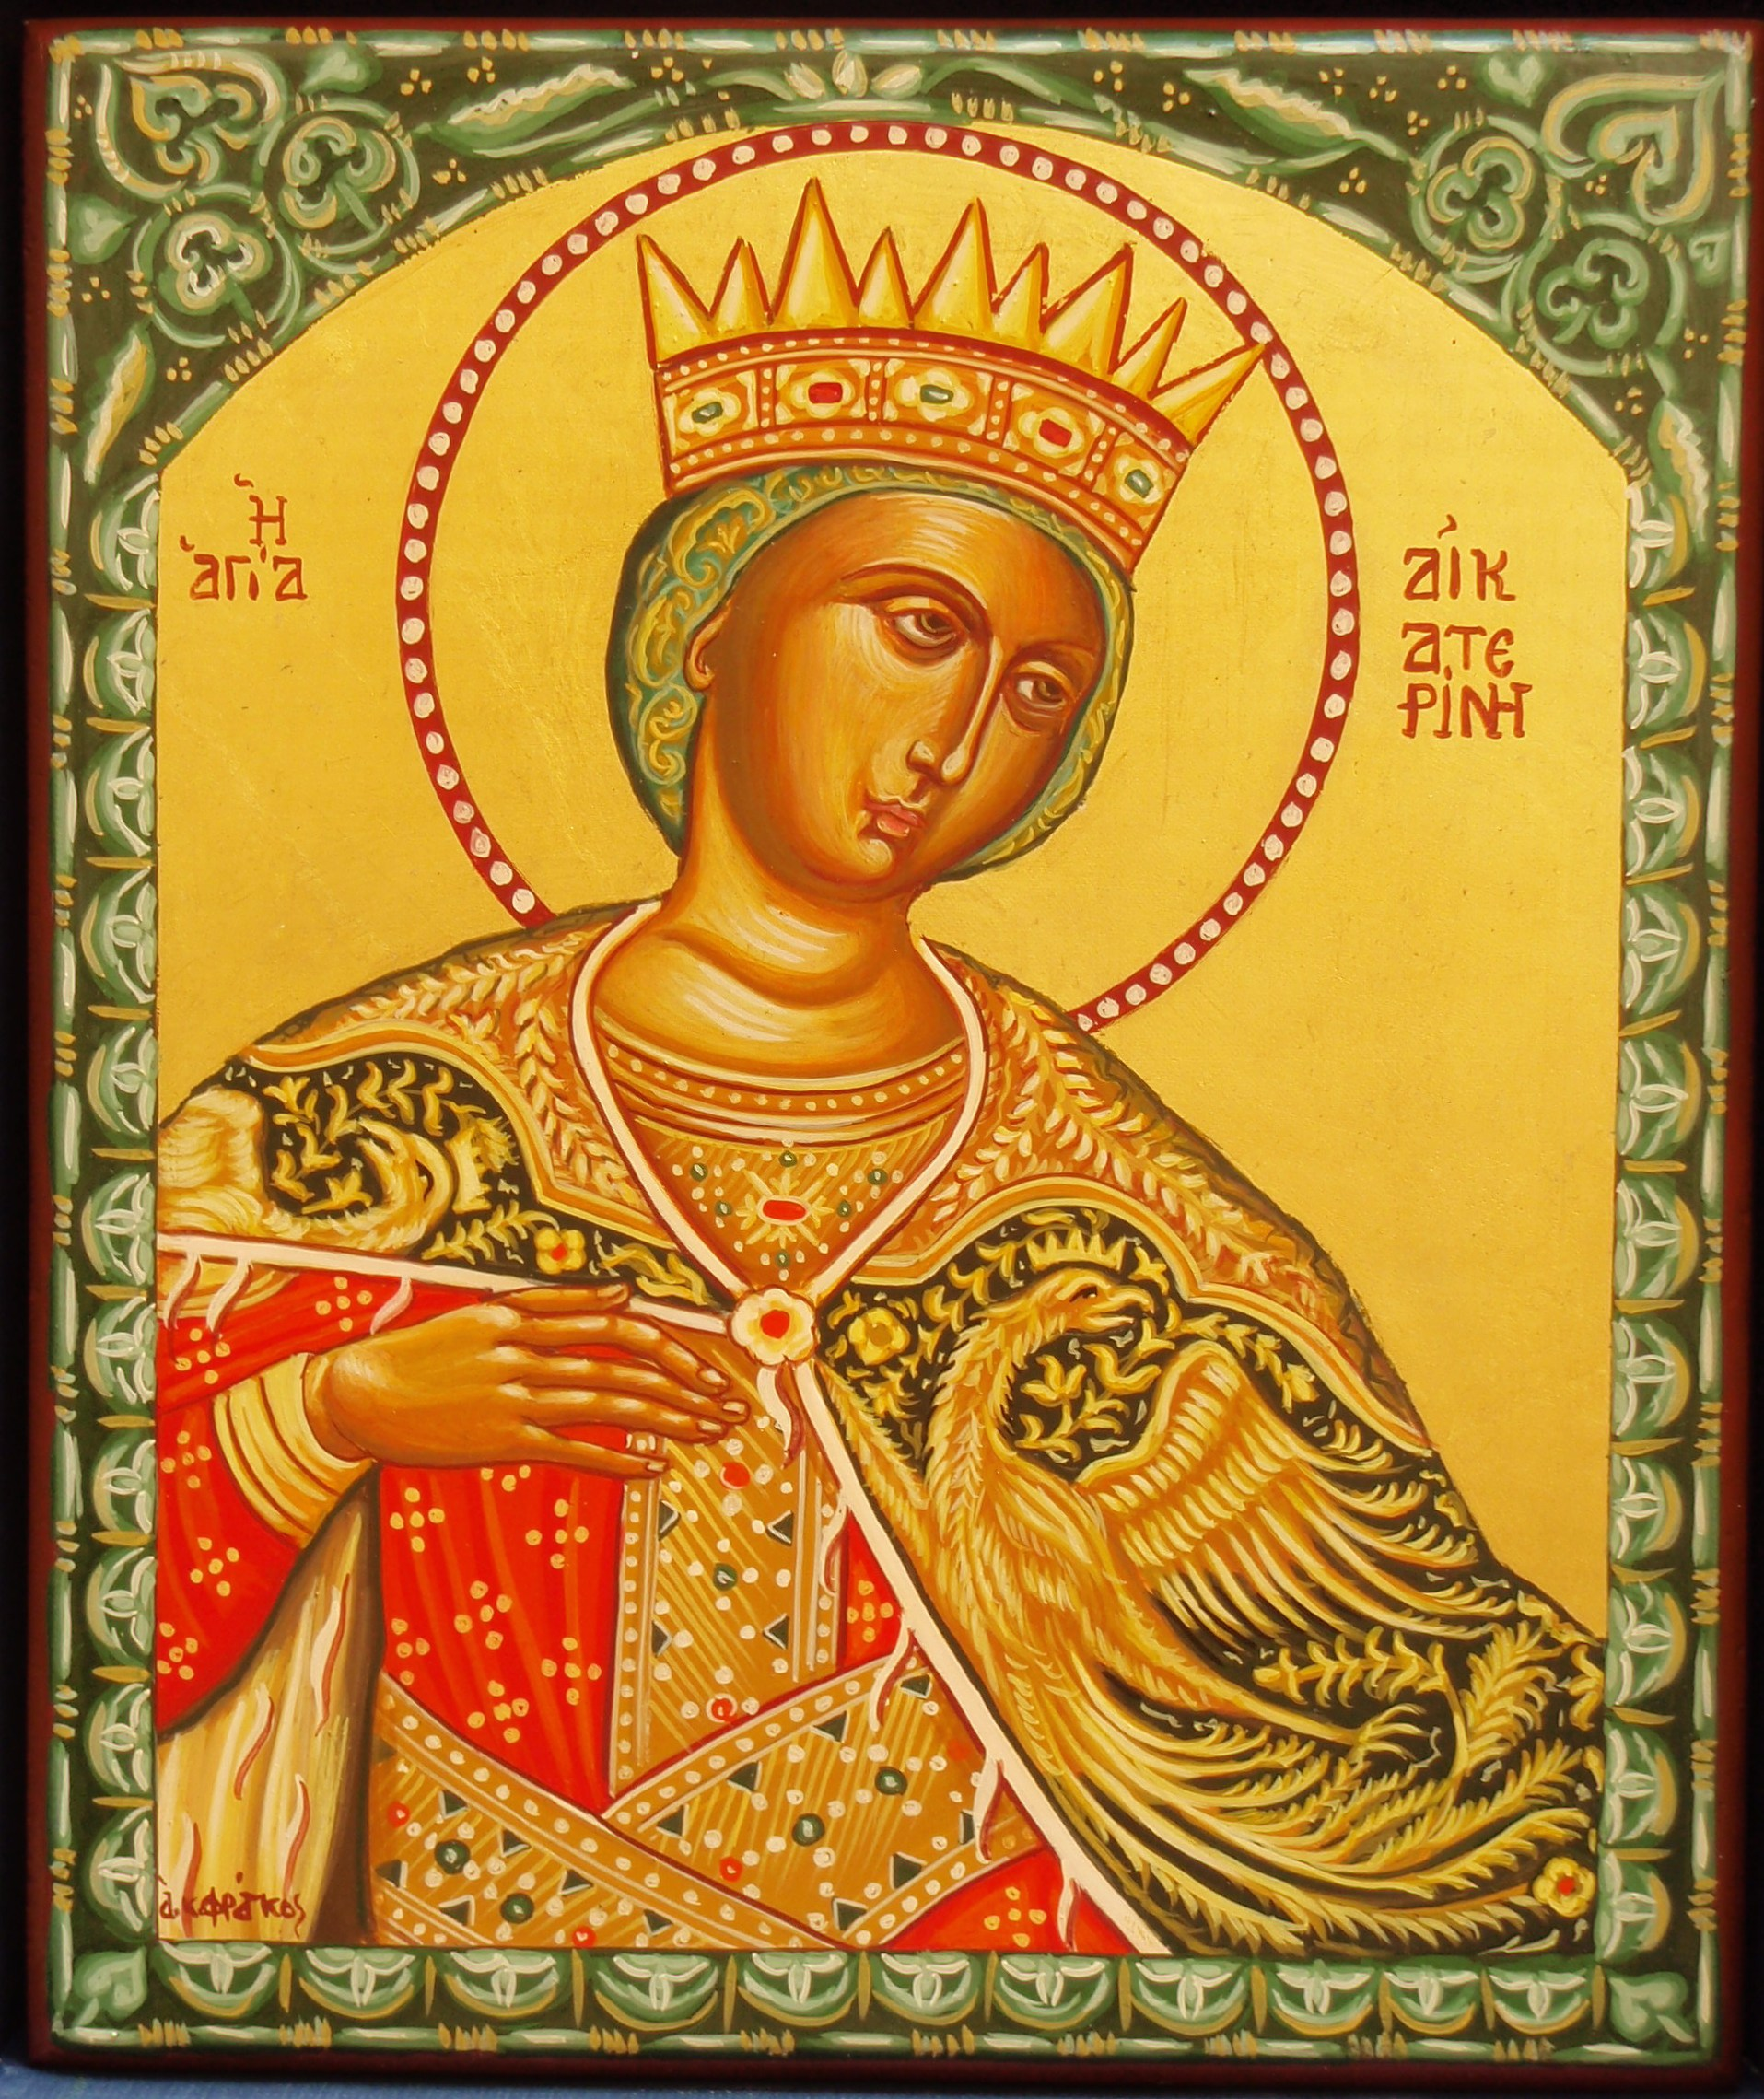
\includegraphics[width=0.5\textwidth]{Katherine1.jpg}}
\date{}
\author{}

\begin{document}
\maketitle
\pagestyle{empty} % Don't show page numbers
\instruction{This page intentionally left blank}
\cleardoublepage
\pagestyle{plain}
\setcounter{page}{1} % Set the page counter to 1 on the first real page
\chapter*{Service of Typica on Sunday, July 26}
\instruction{The Holy Righteous Martyr Paraskeva of Rome \& Seventh Sunday of Matthew:
Hieromartyrs Hermolaus, Hermippus, and Hermocrates of Nicomedia; Venerable Gerontios,
first settler of St. Anne skete on Athos; Moses the Hungarian; Sabbas III, archbishop of Serbia;
Priest Jacob Netsvetov, enlightener of the peoples of Alaska}

\readerline{\throughtheprayers{}}
\choralresponse{./Z-Responses/Obikhod/Amen.ly}

\trisagionNeedsAmen[reader]

\choralresponse{./Z-Responses/Obikhod/Amen.ly}


\centeredsection{The First Antiphon}
\lilypondfile{./Liturgy/B-FirstAntiphon/BlessTheLord_Greek-Music.ly}

\centeredsection{The Second Antiphon}
\lilypondfile{./Liturgy/C-SecondAntiphon/PraiseTheLord_Greek-Music.ly}

\centeredsection{The Third Antiphon}
\lilypondfile{./Liturgy/D-ThirdAntiphon/Beatitudes_Moscow-Music.ly}

\centeredsection{The Epistle}

\instruction{Both of the New Testament lessons are read
without liturgical introduction or conclusion.
The readers start with “The Reading from…” and proceeds}

\paragraph{The Reading from the Epistle of St. Paul to the Galatians. (3:23-4:5)}\mbox{}\\

\begin{maybetwocolumns}
  Brethren, before faith came, we were confined under the Law, kept under restraint until faith
  should be revealed. So that the Law was our custodian until Christ came, that we might be
  justified by faith. But now that faith has come, we are no longer under a custodian; for in Christ
  Jesus you are all sons of God, through faith. For as many of you as were baptized into Christ have
  put on Christ. There is neither Jew nor Greek, there is neither slave nor free, there is neither
  male nor female; for you are all one in Christ Jesus. And if you are Christ’s, then you are
  Abraham’s offspring, heirs according to promise. I mean that the heir, as long as he is a child,
  is no better than a slave, though he is the owner of all the estate; but he is under guardians and
  trustees until the date set by the father. So with us; when we were children, we were slaves to
  the elemental spirits of the universe. But when the time had fully come, God sent forth His Son,
  to redeem those who were under the Law, so that we might receive adoption as sons.
\end{maybetwocolumns}

\centeredsection{The Gospel}

\instruction{Both of the New Testament lessons are read
without liturgical introduction or conclusion.
The readers start with “The Reading from…” and proceeds}

\paragraph{The Reading from the Holy Gospel according to St. Matthew. (9:27-35)}\mbox{}\\

\begin{maybetwocolumns}
  At that time, as Jesus passed on from there, two blind men followed him, crying aloud:
  “Have mercy on us, Son of David.” When He entered the house, the blind men came to Him; and
  Jesus said to them, “Do you believe that I am able to do this?” They said to Him, “Yes, Lord.”
  Then He touched their eyes, saying, “According to your faith be it done to you.” And their eyes
  were opened. And Jesus sternly charged them, “See that no one knows it.” But they went away
  and spread His fame through all that district. As they were going away, behold, a dumb demoniac
  was brought to Him. And when the demon had been cast out, the dumb man spoke; and the crowds
  marveled, saying, “Never was anything like this seen in Israel.” But the Pharisees said, “He casts
  out demons by the prince of demons.” And Jesus went about all the cities and villages, teaching in
  their synagogues and preaching the gospel of the kingdom, and healing every disease and every
  infirmity.
\end{maybetwocolumns}

\centeredsection{Troparia Before the Creed}
\instruction{Plain reading}
\begin{reader}
\item[Reader 1:] The heavenly choir singeth thy praises, saying:
  Holy, holy, holy, Lord of Sabaoth; heaven and earth are full of Thy glory.

\item[Reader 2:] \emph{Come unto him, and be enlightened,
               and your faces shall not be ashamed.}
  The heavenly choir singeth thy praises, saying:
  Holy, holy, holy, Lord of Sabaoth; heaven and earth are full of Thy glory.

\item[Reader 1:] \emph{\glory}
  The choir of the holy angels and archangels,
  with all the powers of heaven, singeth thy praises, saying:
  Holy, holy, holy, Lord of Sabaoth; heaven and earth are full of Thy glory.

\item[Reader 2:]\emph{\nowandever}
\end{reader}

\centeredsection{The Creed}
\input{Common/TheCreed.txt}


\centeredsection{Prayer of Forgiveness}
\readerline{Forgive, remit, pardon, O God, our sins,
  both voluntary and involuntary, in deed and in word, in knowledge or in ignorance,
  committed by night or by day, in mind and in thought.
  Forgive us them all, for thou art good and lovest mankind.
}

\centeredsection{The Lord’s Prayer}
\input{Common/LordsPrayer.txt}

\readerline{Through the prayers of our holy fathers, Lord Jesus Christ our God, have mercy on us.}
\choralresponse{./Z-Responses/Obikhod/Amen.ly}

\centeredsection{Kontakia for Normal Sudays}
\lilypondfile{./Liturgy/H-Kontakion/OProtectionOfChristians_Tone2ByzChant-Music.ly}

\readerline{\lhmForty}

\readerline{
  O Christ our God, Who art worshipped and glorified at all times at every hour both in
  heaven and on earth; Who art long-suffering and plenteous in mercy and compassion; Who lovest
  the just man and showest mercy upon the sinner; and Who callest all men to repentance through 
  the promise of blessings to come; receive, O Lord, at this very hour our supplications, and direct
  our lives in the way of Thy commandments: sanctify our souls, purify our bodies, set our minds
  aright, cleanse our thoughts; deliver us from all affliction, trouble, and distress; compass us about
  with Thy holy angels, that, guided and guarded by them, we may attain unto the unity of the Faith,
  and to the knowledge of Thine unapproachable glory; for Thou art blessed unto ages of ages. Amen.
}

\begin{reader}
  \item \lhmThree{}\\\emph{\gne{}}
  \item \morehonorablethanthetherubim{}
  \item \throughtheprayers{}
\end{reader}

\begin{maybetwocolumns}
\choralresponse{./Z-Responses/Obikhod/Amen.ly}

\readerline{\blessedbethename{}\thrice{}}

\centeredsection{Psalm 33}
\input{./Psalms/Psalm033-unknowntrans.txt}

\end{maybetwocolumns}

\peopleline{\gne}


\centeredsection{A Homily}
\begin{maybetwocolumns}
\instruction{Bearing Witness by Speaking of Neighbors, Not Enemies: Homily for The Holy Righteous Martyr Paraskeva of Rome and the Seventh Sunday of Matthew in the Orthodox Church
}

Especially in stressful times like the ones we face today, it is tempting to define ourselves over
against other people with whom we disagree. There is obviously a lot about which people argue
today, and too many view others who see this or that issue differently as their enemies, not as
their neighbors. Doing so often leads us to insult and condemn people in ways that only bring
judgment upon ourselves, as Christ taught. (Matt. 5: 22-23) The Lord said that our mouths speak
“out of the abundance” of our hearts, which means that our words reveal the state of our souls.
(Luke 6: 45) That is why we will have to give an account for every idle or careless word “in the
day of judgment. For by your words you will be justified, and by your words you will be condemned.”
(Matt. 12: 36-37)

We often forget the power of the spoken word. Remember that the prologue to John’s gospel refers to
Christ as the Logos, the Word, through Whom everything came into existence. He spoke the universe
itself into being, as Genesis describes. Remember how the pride of those who built the tower of
Babel led to the diversity of languages. The resulting division between peoples and nations was
overcome at Pentecost, when the Holy Spirit enabled the disciples to speak in different tongues so
that Jews from around the world would be drawn to the good news of the Savior.

In today’s gospel reading, Christ restored the sight of two Jewish men who had been blind. They
hoped for a Messiah and obviously thought that the Lord could help them. They were, however, blind
to the truth about Christ, for He was not the nationalistic religious leader they expected to bless
their nation and destroy their enemies. Nonetheless, the Savior restored their sight because they
had at least enough faith to trust that He could do so. Then a demon-possessed man who could not
speak was brought to the Savior. Some of the Fathers of the Church see this man as representing the
Gentiles, who had lost the ability to speak the praise of the one true God because of their
idolatry. That the man had lost the ability to speak is a sign of the Gentiles’ slavery to sin,
which distorted and weakened their ability to embrace the high calling of those created in God’s
image and likeness.

The Lord showed mercy to this man also, casting out the demon and restoring his ability to talk.
The Jews who witnessed the miracle said, “Never was anything like this seen in Israel,” for it went
against their expectations for the Messiah to minister to a Gentile. This was such a shocking scene
that “the Pharisees said, ‘He casts out demons by the prince of demons.’” When the Savior set a
Gentile free from slavery to evil and gave him back the basic human ability to speak in the praise
of God, He exploded the Jews’ assumptions about who was an enemy and who was a neighbor. Some found
it easier to speak blasphemous words about the Lord than to open their own mouths in thanks for Him
helping a fellow human being in such a profound way.

In our time and place, it may be hard for us to understanding how radical it was for the Savior to
deliver and heal a Gentile. We probably take for granted what St. Paul wrote to the Galatians:
“There is neither Jew nor Greek, there is neither slave nor free, there is neither male nor female;
for you are all one in Christ Jesus.” As Gentiles ourselves, we have become “Abraham’s offspring,
heirs according to the promise” extended to all through faith in the Savior. As adopted sons and
daughters of God, it would make no sense for us to accept the view that a person’s ancestry,
nationality, social standing, or sex could make him or her a stranger or an outcast from the mercy
of our Lord. Christ has overcome the dividing force of such human characteristics and made clear
that nothing but a stubborn refusal to embrace His healing can keep us from entering into the joy of
His Kingdom.

Unfortunately, it is still very tempting to think and speak about others in ways that underwrite
precisely such divisions. The prophet Isaiah proclaimed, “Surely the nations are like a drop in a
bucket; they are regarded as dust on the scales.” (Isa. 40:15). Still, however, it is so easy to
become idolaters of kingdoms that are very much of this world and to end up denying Christ in what
we say about other people and in how we live. Of course, we are hardly the first generation to face
such temptations.

Today we commemorate the Holy Righteous Martyr Paraskeva of Rome, who certainly did not live
according to the conventional ways of the world. She gave away all her wealth to the poor,
consecrated her virginity to Christ, and proclaimed Him boldly to the pagan Romans in a time when
the penalty for doing so was torture and death. For refusing to do her patriotic duty of
worshiping the false gods of the Roman Empire, she endured horrible tortures. Twice she was set
free from imprisonment, but she was ultimately beheaded for refusing to abandon Christ after
enduring even more horrible abuse. Saint Paraskeva did not see herself according to the categories
of this world, including the sensibilities of the most powerful empire on earth during her lifetime.
Consequently, she was able to make a brilliant witness for Christ and for the superiority of His
Kingdom to any of the passing orders of a world still enslaved to the fear of death.

Regardless of what opinions we may have about any of the pressing concerns of contemporary culture,
we must all wrestle seriously with the question of whether we think and speak of ourselves, our
neighbors, and especially those with whom we disagree in ways that bear witness to Christ’s
restoration of the human person in the image and likeness of God. That means considering whether we
view any person or group as somehow being shut off from the healing mercy of the Savior Who opened
the mouth of the demon-possessed Gentile so that he could give thanks for his healing. That means
asking whether we have accepted corrupt definitions of ourselves or other people that ultimately
amount to the idolatry of seeing reality through the lens of some narrative of earthly glory.

St. Paraskeva had no interest in worshiping such false gods, for she knew that she served a Lord Who
had already triumphed over them in His glorious resurrection on the third day. He made a mockery of
the pathetic powers of this world, and those who share in His life must not think and speak as
though His Cross were not a trophy of victory over them. If we truly share in His life, then we
must refuse to see anyone who bears His image and likeness, and especially those with whom we
disagree or whom we are inclined to disregard, as anything less than a neighbor who is more worthy
of the Lord’s mercy than we ourselves are as the chief of sinners. (1 Tim 1:15) We must guard
our speech to make sure that we do not speak idle words in which we insult and condemn others, and
thus bring judgment on ourselves.

There is no way around it. Our words reveal the state of our souls. Like St. Paraskeva, let us
bear faithful witness to Christ as we refuse to fall into the idolatry of giving our souls to the
false gods of the corrupt ways of a world that crucified our Lord in the name of an earthly empire.
Many such kingdoms want our allegiance today, and we must resist them all if we are to embrace the
blessed promise that is ours through faith in the Savior Who has made us the adopted sons and
daughters of God. Let us think, speak, and act accordingly.
\end{maybetwocolumns}

\centeredsection{Apolytikion of the Ressurection in Tone 6}
\lilypondfile{./Octoechos/ResurrectionalApolytikion-Tone6-Kazan-Music.ly}

\centeredsection{Megalynarion for Normal Sundays}
\lilypondfile{./Liturgy/S-Megalynarion/ItIsTrulyMeet-Kievan-Music.ly}

\readerline{\throughtheprayers}

\choralresponse{./Z-Responses/Obikhod/Amen.ly}

\end{document}

